% !TeX spellcheck = en_US
\documentclass[french]{yLectureNote}

\title{Mécanique}
\subtitle{Mécanique du point}
\author{Paulhenry Saux}
\date{\today}
\yLanguage{Français}

\professor{S.Deheuvels}%sebastien.deveuhels.irap.omp.eu

\usepackage{graphicx}%----pour mettre des images
\usepackage[utf8]{inputenc}%---encodage
\usepackage{geometry}%---pour modifier les tailles et mettre a4paper
%\usepackage{awesomebox}%---pour les boites d'exercices, de pbq et de croquis ---d\'esactiv\'e pour les TP de PC
\usepackage{tikz}%---pour deiffner + d\'ependance de chemfig
\usepackage{tkz-tab}
\usepackage{chemfig}%---pour deiffner formules chimiques
\usepackage{chemformula}%---pour les formules chimiques en \'equation : \ch{...}
\usepackage{tabularx}%---pour dimensionner automatiquement les tableaux avec variable X
\usepackage{awesomebox}%---Pour les boites info, danger et autres
\usepackage{menukeys}%---Pour deiffner les touches de Calculatrice
\usepackage{fancyhdr}%---pour les en-t\^ete personnalis\'ees
\usepackage{blindtext}%---pour les liens
\usepackage{hyperref}%---pour les liens (\`a mettre en dernier)
\usepackage{caption}%---pour la francisation de la l\'egende table vers Tableau
\usepackage{pifont}
\usepackage{array}%---pour les tableaux
\usepackage{lipsum}
\usepackage{yFlatTable}
\usepackage{multicol}
\newcommand{\Lim}[1]{\lim\limits_{\substack{#1}}\:}
\renewcommand{\vec}{\overrightarrow}
\newcommand{\norm}[1]{||\vec{#1}||}
\begin{document}

%\titleOne
\setcounter{chapter}{1}
	\chapter{Cinématique, forces, équilibre }

\section{Rappel de géométrie vectorielle}

\subsection{Coordonnées et composantes}
Soit M un point de l'espace muni du repère $R(O,\vec{e_x}, \vec{e_y},\vec{e_z})$. $\vec{OM} = a\vec{e_x}+ b\vec{e_y}+c\vec{e_z}$.

Les quantités scalaires $x,y$ et $z$ sont les coordonnées du point $M$ dans le repère $R$. On écrit $M(x,y,z)_R$.

Tout vecteur $\vec{u}$ peut se décomposer comme $\vec{u} = u_x\vec{e_x}+ u_y\vec{e_y}+u_z\vec{e_z}$

Les scalaires $u_x,u_y,u_z$ sont appelées composantes du vecteur $\vec{u}$ dans le repère $R$. On écrit $\vec{u} (u_x,u_y,u_z)_R$.

Exercice 2.2.2

\subsection{Produit scalaire et norme}
\subsubsection{Norme}
Si la base $B$ est une base orthonormée directe, alors $||\vec{u}|| = \sqrt{u_x^2+u_y^2+u_z^2}$.
\subsubsection{Produit scalaire entre 2 vecteurs}

\begin{theorem}[Définition]
$\vec{u}\cdot\vec{v} = ||\vec{u}||\times||\vec{v}|| \times \cos(\theta)$.
\end{theorem}
Proriétés du produit scalaire:

\begin{itemize}
 \item C'est un nombre
 \item $\vec{u}\cdot\vec{u} = ||\vec{u}||^2$
 \item $ \vec{u} \perp  \vec{v} = 0$
 \item Il est commutatif : $\vec{u}\cdot\vec{u} = \vec{v}\cdot\vec{u}$ car $\cos(\theta) = \cos(-\theta)$.
 \item Il est bilinéaire : $(\lambda \vec{u}+\beta \vec{v})\cot \vec{w} = \lambda \vec{u}\cdot \vec{w} + \beta \vec{v}\cdot \vec{w}$.
 \item Dans une BOND, on a $\vec{e_i}\cdot\vec{e_j} = \delta_{ij} (= 0 \iff i\neq j \vee = 1 \iff i=j)$.
 \item Dans une BOND : $\vec{u}\cdot\vec{u} = u_xv_x + u_yv_z+u_zv_z$
\end{itemize}
\subsection{Projection sur une base}
\subsubsection{Méthode 1}

Soit un vecteur $\vec{u} = u_x\vec{e_x}+ u_y\vec{e_y}+u_z\vec{e_z}$. On peut retrouver les composantes du vecteur en effectuant le produit scalaire entre ce vecteur et les vecteurs de la base.

$\vec{u}\cdot\vec{e_x} =  u_x$. De m\^eme, $\vec{u}\cdot\vec{e_y} =  u_y$ et $\vec{u}\cdot\vec{e_z} =  u_z$. On peut donc écrire $\vec{u} = (\vec{u}\cdot\vec{e_x})\cdot \vec{e_x} + (\vec{u}\cdot\vec{e_y})\cdot \vec{e_y} + (\vec{u}\cdot\vec{e_z})\cdot \vec{e_z}$.

\checkInfo{Exemple en 2D}{

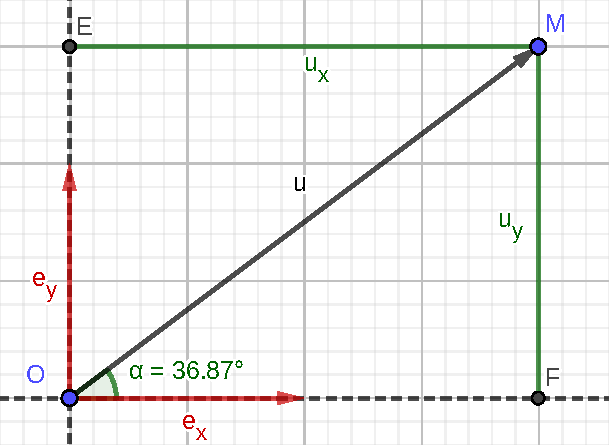
\includegraphics[scale=0.5]{TD2-fig1}

$u_x = \vec{u}\cdot \vec{e_x} = \norm{u}||\vec{e_x}||\cos\theta = ||\vec{u}||\cos\theta$

$u_y = \vec{u}\cdot \vec{e_y} = ||\vec{u}||||\vec{e_y}||\cos(\frac{\pi}{2}- \theta) = ||\vec{u}||\sin(\theta)$}
\subsubsection{Méthode 2}
Projeter $\vec{u}$ dans la base revient à écrire $\vec{u}$ sous la forme $\vec{u} = u_x\vec{e_x}+ u_y\vec{e_y}$ et déterminer $u_x,u_y$. On se place dans un triangle rectangle du schéma précédant

On utilise les relations de trigonométrie : $u_x = ||\vec{u}||\cos(\theta)$ et $u_y = ||\vec{u}||\sin(\theta)$
\subsection{Produit vectoriel}
Soit 2 vecteurs $\vec{u}$ et $\vec{v}$. Le produit vectoriel de $\vec{u}$ et $\vec{v}$, noté $\vec{u} \wedge \vec{v} = \vec{w}$ est l'unique vecteur tel que :

$\vec{w} \perp \vec{u}$ et $\vec{w} \perp \vec{v}$

de norme $\norm{w} = \norm{u} \times \norm{v} \times |\sin(\theta)|$ avec $\theta$ l'angle entre $\vec{u}$ et $\vec{v}$.

De plus, l'ensemble $(\vec{u},\vec{v},\vec{w})$ est une base directe.

$\vec{w}$ est unique car on a défini sa direction, sa norme et son sens.\marginInfo{Sur le sens du produit dans une BOND}{Quand on le fait de gauche à droite, le produit est positif, dans le cas contraire, il est négatif.}

\subsubsection{Calcul avec les coordonnées}

Le produit vaut $\vec{u}\wedge \vec{v}=\begin{pmatrix}
u_yv_z-u_zv_y\\
u_zv_x-u_xv_z\\
u_xv_y-u_yv_x
\end{pmatrix}$

\checkInfo{Méthode du Gamma}{
    On écrit côte à côte les deux vecteurs ${\displaystyle {\vec {u}}}$ et ${\displaystyle {\vec {v}}}$ dont on veut faire le produit vectoriel.

    On réécrit $u_x$ en-dessous de $u_z$ et $v_x$ en-dessous de $v_z$

	Pour avoir les coordonnée $x$, on cache les coordonnées suivant x et on fait le ``calcul en ${\displaystyle \gamma }$.

    Pour obtenir les autres coordonnées, on procède de la même manière.

    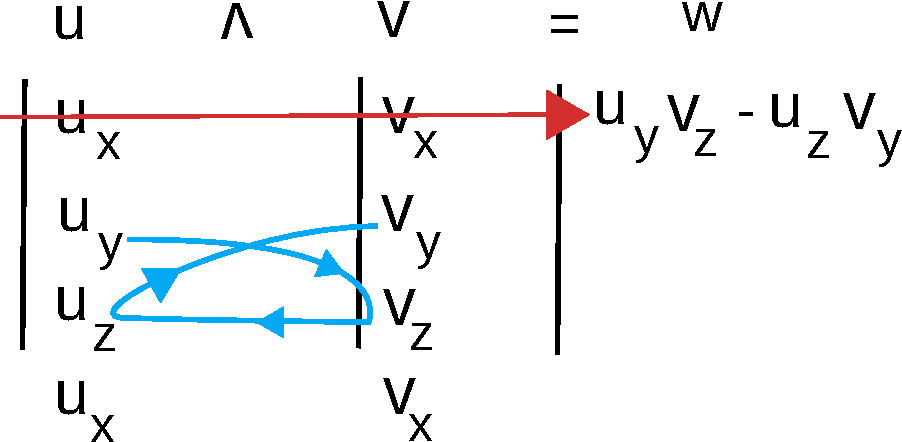
\includegraphics[scale=0.2]{pv1}
    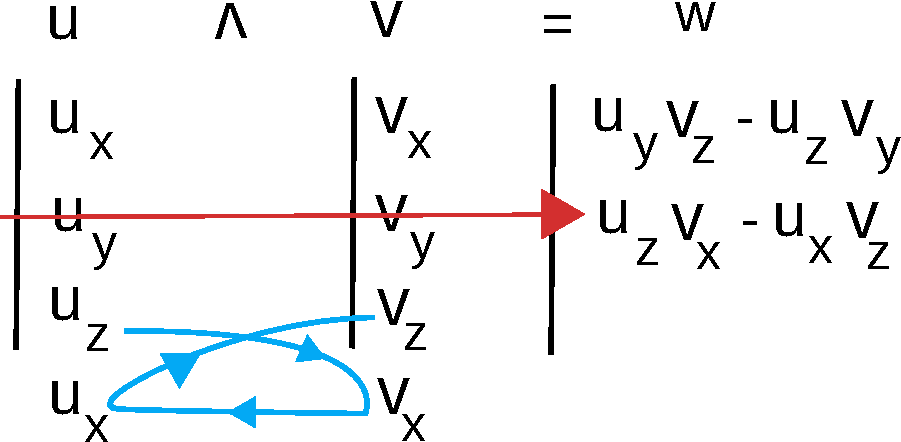
\includegraphics[scale=0.2]{pv2}
    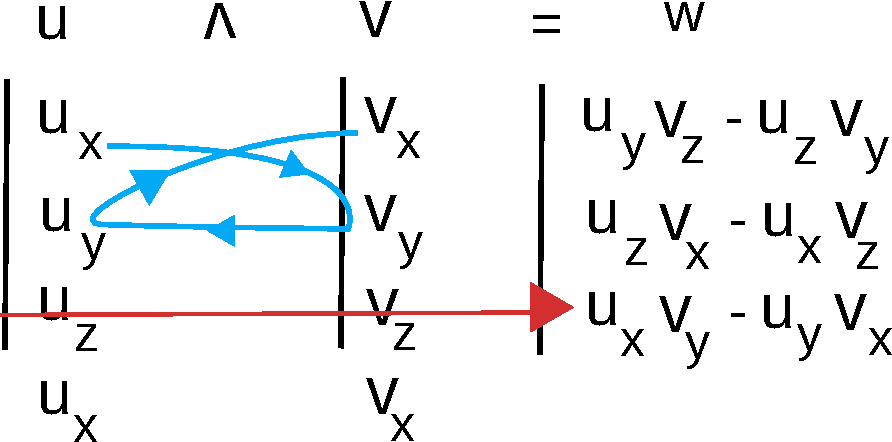
\includegraphics[scale=0.2]{pv3}
    }

\section{Cinématique}
C'est l'étude du mouvement sans ses causes.
\subsection{vecteur position}
Soit un point M de l'espace repéré par rapport à un repère R composée d'une BOND. Il représente la position du centre de masse de l'objet. Il dépend du temps car la position de M varie au cours du temps.

Le vecteur $\vec{OM(t)} = x_m(t)\vec{e_x} + y_m(t)\vec{e_y} + z_m(t)\vec{e_z}$

Les quantités $x_m(t), y_m(t) et z_m(t)$ sont les équations horaire du mouvement. Ce sont des équations paramétriques qui indiquent quel mouvement va suivre $M$. On peut en déduire l'équation cartésienne de la trajectoire en supprimant la dépendance au temps

\subsection{Vecteur vitesse}
\warningInfo{Direction du vecteur vitesse}{Le vecteur vitesse est toujours tangent à la trajectoire et dans le sens du mouvement}
\subsubsection{Composantes du vecteur vitesse}

\begin{flalign*}
\vec{v_{M/R}} = \dot{x}_m(t)\vec{e_x} + \dot{y}_m(t)\vec{e_y} + \dot{z}_m(t)\vec{e_z}
\end{flalign*}
\subsection{Vecteur accélération}
\begin{flalign*}
\vec{a_{M/R}} &=  \frac{d\vec{v(t)}}{dt}\\
&= \frac{d^2\vec{OM(t)}}{dt^2}
\end{flalign*}
\warningInfo{Direction du vecteur accélération}{Dans le cas général, il n'est pas tangent à la trajectoire.}

\subsubsection{Composantes du vecteur accélération}
\begin{flalign*}
\vec{a_{M/R}} = \ddot{x}_m(t)\vec{e_x} + \ddot{y}_m(t)\vec{e_y} + \ddot{z}_m(t)\vec{e_z}
\end{flalign*}
\subsection{Changement de référentiel dans le cas d'une translation}
Soit 2 référentiels R et R' tels que R' est une translation rectiligne par rapport à R avec une vitesse $\vec{V_{R'/R}}$

Dans ce cas on a $\vec{V_{M/R}} = \vec{V_{M/R'}} + \vec{V_{R/R'}}$. C'est la loi de composition des vitesses.

\subsection{Types de mouvements}
\subsubsection{Mouvement uniforme}
Mouvement pour lequel $\norm{V_{M/R}}$ est constant.

\warningInfo{Implications fausse}{Ne veut pas dire que le vecteur vitesse est constant ou que le vecteur accélération est nul (voir orbite de la terre dans le repère de Frenet)}

On a un mouvement uniforme si $\vec{v}\cdot \vec{a} = 0$, donc que $\vec{a}\perp\vec{a}$.

Conséquences :

Si $\vec{v}\cdot\vec{a} > 0$ alors $\frac{d\norm{V_{M/R}}}{dt} > 0$ et $\norm{V_{M/R}}$ augmente au cours du temps (mouvement accéléré).

Si $\vec{v}\cdot\vec{a} < 0$ alors $\frac{d\norm{V_{M/R}}}{dt} < 0$ et $\norm{V_{M/R}}$ diminue au cours du temps (mouvement décéléré).

$\vec{v}\cdot\vec{a} > 0$ si $\cos \alpha > 0 \iff \alpha \in [-\frac{\pi}{2},\frac{\pi}{2}]$.

$\vec{v}\cdot\vec{a} < 0$ si $\cos \alpha < 0 \iff \alpha \in [\frac{\pi}{2},\frac{3\pi}{2}]$.
\section{Rappels sur les lois de Newton}
\subsection{Référentiel galiléen}
C'est un référentiel dans lequel un système isolé (pas de forces) ou pseudo-isolé (résultante des forces nulle) est au repos ou en mouvement rectiligne uniforme (principe d'inertie). C'est un idéal vers lequel on peut tendre mais qu'on atteint pas.

\subsubsection{Référentiel géocentrique}
L'origine est le centre de la Terre avec les axes pointés vers des étoiles lointaines ($\simeq$ fixe) mais il est en rotation autour du Soleil, donc considéré comme galiléen si le temps du mouvement est petit par rapport à une année.
\subsubsection{Référentiel de Copernic}
L'origine est le centre de gravité du système solaire mais aussi en rotation autour du centre de la galaxie $250\cdot10^6$ans.
\subsection{Lois de Newton}
\subsubsection{Principe d'inertie}
Il existe un certain type de référentiels, dits galiléens, dans lesquels ces principes s'appliquent.
\subsubsection{Principe fondamental de la dynamique}
Il s'exprime à partir de la quantité de mouvement $\vec{p_{M/R}} = m\vec{v}$ :

\begin{theorem}[Relation]
\[\frac{d\vec{p_{M/R}}}{dt} = \sum_i \vec{F_i}\]
\end{theorem}

Dans la pratique, la masse du système est souvent constante, dans ce cas :

\begin{theorem}[Relation]
\[\frac{d\vec{p_{M/R}}}{dt} = m\frac{d\vec{v_{M/R}}}{dt} =  m\vec{a} = \sum_i \vec{F_i}\]
\end{theorem}
\subsubsection{Principe d'action réciproque}
La force exercée par A sur B vaut l'opposée de la force exercée par B sur A : $\vec{F_{A/B}} = - \vec{F_{B/A}}$.
\subsection{Exemples de forces}
\subsubsection{Force gravitationnelle}
C'est la première intéraction fondamentale

Soit 2 corps de masse $m_A$ et $m_B$. On a :
\[\vec{F_{g,A/B}} = -G\frac{m_Am_B}{d^2} \vec{e_r}\]

\checkInfo{Remarque}{Dans le contexte de la relativité générale, le concept de force gravitationnelle est remplacé par une courbure de l'espace-temps produite par des objets massifs. }
\subsubsection{Force électrostatique ou force de Coulomb}

Soit 2 charges $q_A$ et $q_B$, distante de $r$. On a, avec $\epsilon_0$ la permittivité du vide :
\[\vec{F_{e,A/B}} = k_e\frac{q_Aq_B}{r^2} \vec{e_r} = \frac{q_Aq_B}{4\pi \epsilon_0r^2} \vec{e_r}\]

Si les 2 charges sont de m\^eme signe, la force est répulsive, dans la cas contraire, elle est attractive.

À l'échelle des particules, cette force domine sur la force gravitationnelle.

\subsubsection{Poussée d'Archimède}

\begin{theorem}[Expression de la poussée d'Archimède]
Tout corps plongé dans un fluide (gaz ou liquide) est soumis à une force, appelée poussée d'Archimède qui à la m\^eme direction que le poids, de sens opposé et dont la norme est égale au poids du volume de fluide déplacé.
\end{theorem}
 \subsection{Équilibre statique}
 Dans un référentiel galiléen, le principe d'inertie s'applique t on a l'équivalence $\sum_i \vec{F_i} = \vec{0} \iff \vec{a} = \vec{0}$. Le système est au repos ou en mouvement rectiligne uniforme

\section{Frottements solides}
\subsection{Approche phénoménologique}
\begin{theorem}[Définition]
Elles sont liée au contact entre 2 surfaces
\end{theorem}
Le bilan des forces est $\vec{P},\vec{F},\vec{R}$ et on a : $\vec{P}+\vec{F}+\vec{R} = \vec{0}$ On aura donc nécessairement pour $\vec{R}$
\begin{itemize}
 \item une composante normale $\vec{N}$ qui s'oppose au poids
 \item une composante tangentielle $\vec{T}$ qui s'oppose à $\vec{F}$. Elle correspond aux forces de frottement solide et dépend des matérieux des surfaces en contact
\end{itemize}
Si la norme de $\vec{F}$ augmente, l'objet finit par se mettre en mouvement.

\subsection{Lois de Coulomb}
Elles sont empirique, i.e déduites de l'expérience. La réaction du support est décomposée en $\vec{R} = \vec{T}+\vec{N}$
\begin{theorem}[Lois]
\begin{itemize}
 \item Il y a équilibre si $\norm{T} \leq \mu_s \norm{N}$
 \item Si il y a un glissement, $\norm{T} = \mu_d \norm{N}$ et $\vec{T}$ dans la direction opposé au mouvement, c'est à dire : $\vec{T} = -\norm{T}\times \frac{\vec{v}}{\norm{v}}$.
\end{itemize}
\end{theorem}
\end{document}

